\chapter{Teoría}

La luz, al pasar de un medio lineal, homogéneo e isótropo a otro medio material con las mismas características, se descompone en dos haces: uno reflejado y otro transmitido. Para calcular la intensidad de los haces reflejado y transmitido se emplean las fórmulas de Fresnel. En su deducción se consideran las condiciones de frontera impuestas por las ecuaciones de Maxwell sobre los campos electromagnéticos (EMs), de las que se deduce, además, la dirección de propagación de los haces separados.  Una vez, determinadas las condiciones de frontera de los campos EMs y la dirección de propagación de la luz, se calcula la relación  entre los campos eléctricos evaluados en la frontera entre ambos medios, resultando en los \emph{coeficientes de amplitud}. Finalmente, la conservación de la energía que es considerada, resultando en las ecuaciones de Fresnel.


\section{Fórmulas de Fresnel}

% \index{MaxEqs@Ecuaciones de Maxwell}
Las ecuaciones de Maxwell en su forma diferencial son   \cite{griffiths2013electrodynamics}  \index{MaxEqs!forma diferencial}
	\begin{subequations} \label{eqs:Maxwell}
	\begin{tcolorbox}[title = Ecuaciones de Maxwell (Forma diferencial),
	ams align ]
	\nabla \cdot\vb{E} &= \frac{\rho_{tot}}{\varepsilon_0}, &\mbox{(Ley de Gauss eléctrica)}  
	\label{seq:GE} \\
	\nabla \cdot\vb{B} &= 0,						&\mbox{(Ley de Gauss magnética)}   
	\label{seq:GM} \\
	\nabla \times\vb{E} &= -\pdv{\vb{B}}{t}, 	&\mbox{(Ley de Faraday-Lenz)}		
	\label{seq:FL}\\
	\nabla \times\vb{B} &= \mu_0 \vb{J}_{tot} +\varepsilon_0\mu_0 \pdv{\vb{E}}{t}, &
	\mbox{(Ley de Ampère-Maxwell)} \label{seq:AM}
	\end{tcolorbox}\end{subequations}\vspace*{-1em}\noindent 
donde $\vb{E}$ es el campo eléctrico, $\vb{B}$ el campo magnético, $\rho_{tot}$ es la densidad volumétrica de carga total  y $\vb{J}_{tot}$ la densidad volumétrica de corriente total, $\varepsilon_0$ la permitividad eléctrica del vacío y $\mu_0$ la permeabilidad magnética del vacío.
%
%Aplicando el teorema de la divergencia\footnote{\setstretch{1.0}Teorema de la divergencia:  $\int_V \nabla \cdot \vb{A} pdv = \oint_{\partial V} \inner{A}{da}$, con $\vb{A}$ un campo vectorial de clase $C^2$ en un volumen $V$.} y el teorema de Stokes\footnote{\setstretch{1.0}Teorema de Stokes: $\int_S \nabla \times\vb{A}\cdot \vb{da} = \oint_{\partial S} \inner{A}{dl}.$, con $\vb{A}$ un campo vectorial de clase $C^2$ en una superficies orientable $S$.} a las Ecs. \eqref{eqs:MDif} se obtienen las ecuaciones de Maxwell en forma integral \cite{griffiths2013electrodynamics}:\index{MaxEqs!forma integral}
%	\begin{subequations}	\label{eqs:MInt}
%	\begin{tcolorbox}[ title = Ecuaciones de Maxwell (Forma integral), ams align]
%	\oint_{S_c} \vb{E}\cdot\vb{\dd a}  &= \frac{Q_{tot}^{\,enc}}{\varepsilon_0},\label{eq:GEint}\\
%	\oint_{S_c} \vb{B}\cdot\vb{\dd a}  &= 0,\label{eq:GMint} \\
%	\oint_C \vb{E}\cdot\vb{\dd a} & =-\dv{}{t}\int_S \vb{B}\cdot\vb{\dd a},\label{eq:FLint}\\
%	\oint_C \vb{B}\cdot\vb{\dd l} &=\mu_0 I_{tot}^{atr} +\varepsilon_0\mu_0 \dv{}{t} \int_S 	
%	\vb{E}\cdot\vb{\dd a}  \label{eq:AMint}
%	\end{tcolorbox}\end{subequations}\noindent
%%		\begin{subequations}	\label{eqs:MInt}
%%	\begin{tcolorbox}[ title = Ecuaciones de Maxwell (Forma integral)]
%%	\eqhalf{\oint_{S_c} \vb{E}\cdot\vb{\dd a}  = \frac{Q_{tot}^{\,enc}}{\varepsilon_0},\label{eq:GEint}}
%%	\eqhalf{\oint_{S_c}\vb{B}\cdot\vb{\dd a} = 0,\label{eq:GMint} }
%%	\eqhalf{\oint_C \vb{E}\cdot\vb{\dd l}   =-\dv{}{t}\int_S \inner{B}{da},\label{eq:FLint}}
%%	\eqhalf{\oint_C \vb{B}\cdot\vb{\dd l}  =\tilde{\mu}_0 I_{tot}^{atr} +\varepsilon_0\tilde{\mu}_0 \dv{}{t} \int_S 	\vb{E}\cdot\vb{\dd a}  \label{eq:AMint}}
%%	\end{tcolorbox}\end{subequations}\noindent		
%con $S_c$ una superficie cerrada, $S$ una superficie abierta y $C$ la frontera de $S$. El término $Q_{\,tot}^{enc}$ es la carga total encerrada por $S_c$ y el término $I_{tot}^{atr}$ es la corriente total que atravieza el área encerrada por $C$.

Al sustituir las ecuaciones de Maxwell en la expresión de la fuerza de Lorentz, que es la fuerza ejercida sobre una partícula con carga $q$ y velocidad $\vb{v}$ en presencia de campos EM \cite{griffiths2013electrodynamics}, dada por $	\vb{F} = q \left( \vb{E} + \vb{v}\times \vb{B} \right)$,\index{Fuerza de Lorenz} se deduce el teorema de  conservación de la energía \cite{griffiths2013electrodynamics}. De éste, se define el vector de Poynting $\vb{S}$\index{Vector de Poynting}, correspondinte al flujo de energía por unidad de tiempo, por unidad de área, transportado por los campos EMs \cite{griffiths2013electrodynamics}, dado por la expresión  
	\begin{tcolorbox}[title = Vector de Poynting, ams align]
	\vb{S} = \frac{1}{\mu}_0 \vb{E}\times\vb{B}.  \label{eq:Poynting}
	\end{tcolorbox}

Los campos EMs, al desacoplar las ecuaciones de Maxwell, obedecen la ecuación de onda \cite{algo}. Una solución a esta ecuación se obtiene al emplear la transformada Fourier\footnote{ \setstretch{1.0} $\mathcal{F}[f(\vb{r},\omega)] = \int_{-\infty}^\infty f(\vb{r},t) e^{i(\vb{k}\cdot\vb{r} -\omega t)} dt$, con $\omega$ una función de $\vb{k}$. La transformada de Fourier inversa es entonces $\mathcal{F}^{-1}[f(\vb{r},t)] =\frac{1}{2\pi} \int_{-\infty}^\infty f(\vb{r},t) e^{i(\vb{k}\cdot\vb{r} -\omega t)} d\omega$.} \cite{jackson1999electrodynamics}, proceso que concluye con ondas planas como soluciones , es decir, 
	\begin{subequations}
	
	\eqhalf{	\vb{E}(\vb{r},t) =\vb{E_0}e^{i(\vb{k}\cdot\vb{r} \,-\,\omega \,t)},\label{seq:OplanaE} }
	\eqhalf{	\vb{B}(\vb{r}, t) =\vb{B_0}e^{i(\vb{k}\cdot\vb{r} \,-\,\omega\, t)}, \label{seq:OplanaB}}
	\label{eqs:OPlana}\end{subequations} 
	
\vspace*{-1em}\noindent 
en donde  $\vb{E}_0$ y $\vb{B}_0$ son las amplitudes de las ondas EMs, $\vb{k}$ es el vector de onda y $\omega$ es la frecuencia angular; la triada de vectores \{$\vb{k},\, \vb{E},\, \vb{B}$\} constituye una base ortogonal derecha en el vacío \cite{griffiths2013electrodynamics}. 

Para que las ondas planas sean solución de las ecuaciones de Maxwell, se impone la \emph{relación de dispersión}, que forza a  la magnitud del vector de onda $k$ y la frecuencia angular $\omega$ a obedecer la expresión 
	\begin{tcolorbox}[title = Relación de dispersión, ams align]
	\omega = c k \label{eq:dispersion}
	\end{tcolorbox}\vspace*{-1em}\noindent
en donde  $c$ es la velocidad de la luz. 

El medio por el que se propaga la luz está caracterizado por  la permitividad eléctrica $\tilde{\varepsilon}$ y la permeabilidad magnética $\tilde{\mu}$ del material y el índice de refracción $n$. Estas cantidades se relacionan según la ecuación 
	\begin{tcolorbox}[title = Índice de refracción, ams align]
	n = \sqrt{\frac{\tilde{\varepsilon} \tilde{\mu}}{\varepsilon_0 \mu}_0}=\sqrt{ \varepsilon \mu},\label{eq:indice} 
	\end{tcolorbox}\vspace*{-1em}\noindent
donde $\varepsilon = \tilde{\varepsilon}/\varepsilon_0$ es la permitividad eléctrica relativa, también conocida como función dieléctrica, y $\mu = \tilde{\mu}/\mu_0$ la permeabilidad magnética relativa. Tanto $n$, como $\varepsilon$ y $\mu$ se determinan de forma experimental y son, en general, cantidades complejas.

Las ecuaciones de Maxwell imponen constricciones sobre los campos EMs cuando estos cruzan la frontera entre dos medios distintos, denominada interfaz (ver Fig. \ref{fig:GaussAmpere}). En su deducción, los campos EMs son evaluados sobre la interfaz al calcularlos en una región en el espacio infinitesimalmente chica para que sean considerados constantes. Si los medios son lineales, homogéneos e isótropos, y no hay cargas externas, los campos EMs obedecen las  expresiones \cite{algo} 
	\begin{subequations}
	\begin{tcolorbox}[title = Condiciones de frontera de los campos EM ]
	\eqhalf{\varepsilon_1 E^\perp_1 - \varepsilon_2 E^\perp_2 = 0, \label{seq:Eperp}}
	\eqhalf{E_1^\parallel -E_2^\parallel = 0,\label{seq:Epara}}
	\eqhalf{B_1^{\perp} - B_2^{\perp} = 0, \label{seq:Bperp} }
	\eqhalf{\frac{\vb{B}^\parallel_1}{\mu_1} - \frac{\vb{B}^\parallel_2}{\mu_2} =\vb{0},\label{seq:Bpara}} 
	\end{tcolorbox} \label{eqs:CFrontera}	\end{subequations} \vspace*{-1em}\noindent
en donde el subíndice hace referencia al medio, y $\varepsilon_i$ y $\mu_i$ son la permitividad eléctrica y la permeabilidad magnética que caracterizan al medio.

	\begin{figure}[t!]\centering
	\begin{subfigure}{.05\textwidth}\vspace{-3cm}\caption{}\label{sfig:AmpereLoop}	\end{subfigure}
	\begin{subfigure}{.43\textwidth} \hspace*{-1cm}
\begin{tikzpicture}[scale=.89]
%\draw (3.46,1.9) circle(2pt);ESTA ES LAREFERENCIA PARA ANTES DE MOVER LAS COSAS

%%%%%%%%%%%%%%%%%%%%%%%%%%%%%%%%%%%%%%%%%%%%%%%% 	SUPERFICIE
\shadedraw[	top color =lblue,				%%%%	Color de arriba
			bottom color =lblue,				%%%%	Color de abajo
			middle color = bone, 			%%	Color de en medio
			shading angle = -22]			%%%%	Ángulo de gradiente
			
(-1,1) ..controls (2, 0) and (3,3.5) .. (4.5,3.5) %	Aquí se dan las lineas
-- (7,3.2) .. controls (5,3) and (4,-.5) .. (2.5,.5)%	A .. ctrls P and Q.. B 
--(-1,1);								%%%%%%%%%	P y Q jalan la linea de A a B
\node[color = black] at (3,.5) { $\sigma_{tot}$};
\node  at (0,1.1) {Medio 1};
\node at (0,.5) {Medio 2};

%%%%%%%%%%%%%%%%%%%%%%%%%%%%%%%%%%%%%%%%%%%%%%%%%%%%%%%%%	PILL-BOX
\fill[dgreen, opacity = .3]						%%%%%%%%	Cara del cilindro
 (3.46-.7,2.05) arc(180: 0: .7 and .2)			%%%%%%%% 	se pone el principio pero es
-- (3.46+.7,1.75) arc(0: -180: .7 and .2)		%%%%%%%		lo ultimo que puedo escribir
-- (3.46-.7,2.05);

\draw[black](3.46,2.05) circle (.7 and .2)		%%%%%%		Centro y radios de curvatura
(4.1,2.15)node[above]{ $A$};	%%%%		Etiqueta del área
\fill[dgreen, opacity = .1] (3.46,2.05) circle (.7 and .2); 

\draw[black](3.46,1.9)  circle (.7 and .2);
\fill[dgreen,opacity = .1](3.46,1.9)  circle (.7 and .2);

\draw[densely dotted, black](3.46,1.75)  circle (.7 and .2);
\fill[dgreen,opacity = .1](3.46,1.75)  circle (.7 and .2);

\draw[black, line width = .2mm]						%%%%%%	Lineas que faltó llenar
(3.46-.7,2.05) -- (3.46-.7,1.9)		(3.46+.7,2.05) -- (3.46+.7,1.9);
\draw[densely dotted, black, line width = .2mm]
(3.46-.7,1.9) -- (3.46-.7,1.75)		(3.46+.7,1.9) -- (3.46+.7,1.75);
 
  
%%%%%%%%%%%%%%%%%%%%%%%%%%%%%%%%%%%%%%%%%%%%%%%%%%%%%%%%%%%%	VECTOR NORMAL (Perp)
\draw[ -latex ,line width=.2mm, black]	
 (3.46,2.05)--(3.46,2.6+.1);	%%%%	Se toma un punto medio y se desplaza para dar profundidad
\node[color = black, right] at (3.46-.1,2.6+.2) { $\vb{a}_\perp$};%	Se etiqueta la flecha

%%%%%%%%%%%%%%%%%%%%%%%%%%%%%%%%%%%%%%%%%%%%%%%%%%%%%%%%%%%%	VECTOR NORMAL (Paralelo)
\draw[-latex ,line width=.2mm, black]	
 (3.46-.7+.3, 1.9-.15)-- (3.46-.7-.1,1.95-.4);	
\node[color = black, left] at (3.46-.1,1.95-.6) { $\vb{a}_\parallel$};%	Se etiqueta la flecha

%%%%%%%%%%%%%%%%%%%%%%%%%%%%%%%%%%%%%%%%%%%%%%%%%%%%%%%%%	LINEA DE ALTURA
\draw[|-, line width=.2mm,black]
(3.46+.7+.15,2.05) -- (3.46+.7+.15, 1.9);
\draw[-|, densely dotted, line width=.2mm,black]
(3.46+.7+.15,1.9) -- (3.46+.7+.15,1.7);
\node[color = black, right] at (3.46+.7+.15,1.9) { $\delta$};
\end{tikzpicture}	
	\end{subfigure}
	\begin{subfigure}{.05\textwidth}\vspace{-3cm}\caption{}\label{sfig:GaussSurface}\end{subfigure}
	\begin{subfigure}{.43\textwidth}  \hspace*{-1cm}
\begin{tikzpicture}[scale=.89]
%--------------------------------------------------- 	SUPERFICIE

\shadedraw[	top color =lblue,				%		Color de arriba
			bottom color =lblue,				%		Color de abajo
			middle color = bone, 			%		Color de en medio
			shading angle = -18]			%		Ángulo de gradiente
			
	(-1,1) ..controls (2, 0) and (3,3.5) .. (4.5,3.5) %	Aquí se dan las lineas
	-- (7,3.2) .. controls (5,3) and (4,-.5) .. (2.5,.5)%	A .. ctrls P and Q.. B 
	--(-1,1);								%%%%%%%%%	P y Q jalan la linea de A a B

\node[color = black] at (3,.7) { $\vb{K}_{tot}$};
\node  at (0,1.1) {Medio 1};
\node at (0,.5) {Medio 2};
\draw[- latex, thick]  (2.4,.78)  -- (1.4,.9) ;  
\draw[- latex, thick]  (2.7,.88)  -- (1.7,1) ; 
\draw[- latex, thick]  (3,.98)  -- (2,1.1) ; 

%---------------------------------------------------	CIRCUITO
\draw[densely dotted, line width=.2mm,black, reverse directed] 
(3.0,1.4)-- (3.92,2.4)
		-- (3.92,2.1)
		-- (3.0,1.1)
		-- (3.0,1.4);
\draw[line width=.2mm, black, directed] 
(3.0,1.4)--(3.92,2.4)		 
 		-- (3.92,2.7)		
 		-- (3.0,1.7) 
 		-- (3.0,1.4);
 							%%%%%%%%%	Estos ultimos son para colorear el circuitp
\fill[dgreen,opacity = .3] (3.0,1.4)--(3.92,2.4)-- (3.92,2.7)-- (3.0,1.7)-- (3.0,1.4);
\fill[dgreen,opacity = .2](3.0,1.1)--(3.92,2.1)-- (3.92,2.4)-- (3.0,1.4)-- (3.0,1.1);
 
%---------------------------------------------------	VECTOR NORMAL
\draw[ - latex ,line width=.2mm, black]	
 (3.46,1.9)--(3.46,2.6);	%%%%	Se toma un punto medio y se desplaza para dar profundidad
\path (3.5,2.5) node[color = black, above]{ $\vu{u}$};%	Se etiqueta la flecha

%---------------------------------------------------      LINEA DE LONGITUD
\draw[|-|,line width=.2mm,black] (3.08+.1,1.1-.1)--(4+.1,2.1-.1);%		Se escogieron puntos arbitrarios
\path (3.34+.4 ,1.8-.4) node[color = black]{ $l$}  ;%	Se toma el punto medio y se traslada

%---------------------------------------------------	LINEA DE ALTURA
\draw[|-, densely dotted, line width=.2mm,black] (3.92+.2,2.1+.1)--(3.92+.2,2.4+.1);
\draw[-|, line width=.2mm,black] (3.92+.2,2.4+.1)--(3.92+.2,2.7+.1);
\path (3.92+.2,2.4+.1) node[color = black, right]{ $ \delta$};
\end{tikzpicture}
	\end{subfigure} \vspace*{-.7cm}
	\caption{Esquema de una interfaz entre dos medios distintos y arbitrarios con {\bf a)} una densidad de carga superficial $\sigma_{tot}$ y {\bf b)} una densidad de corriente superficial $\vb{K}_{tot}$. El vector normal al cilindro en \textbf{a)} es $\vb{a}$, $A$ es el área de la base del cilindro y $\delta$ su altura; el vector normal a la interfaz es $\vu{u}$, que define un circuito de largo $l$ y altura $\delta$. En ambas figuras se calculan los campos EMs en el límite $\delta\to 0$.}	\label{fig:GaussAmpere}	
	\end{figure}	
		
		\subsection{Coeficientes de amplitud}		
		
Cuando un haz de luz, modelado por el campo eléctrico de una onda plana [Ec. \eqref{seq:OplanaE}], incide sobre la interfaz entre dos medio lineales, homogéneos e isótropos, este es descompuesto en un haz reflejado y otro transmitido. Ambos haces son modelados por ondas planas que se propagan a través del \emph{plano de incidencia}, definido por la onda plana incidente y el vector normal a la interfaz. Dado que las condiciones de frontera sobre la onda plana incidente y reflejada en el medio de incidencia, caracterizado por el índice de refracción $n_i$, y la onda transmitida, en el medio de transmisión, con índice de refracción $n_t$, son válidas para todo tiempo y todo punto en la interfaz, la fase de las tres ondas son iguales. De esta aseveración se deducen la ley de la reflexión, y ley de Snell\footnote{La ley fue nombrada así debido al físico holandés Willebroerd Snellius aunque investigaciones más recientes indican que el registro más antiguo de esta ley (correctamente formulada) fue en el año 984 en el libro \emph{On the Burning Instruments} del matemático persa Ibn Sahl \cite{kwan2002really}.}, dadas por las expresiones  
	\begin{tcolorbox}[title = Ley de la reflexión y ley de Snell ]
	\eqhalf{\theta_i = \theta_r  \label{eq:LeyReflexion}}
	\eqhalf{ n_i \sin\theta_i = n_t \sin\theta_t,\label{eq:LeySnell}}
	\end{tcolorbox}	 \vspace*{-1em}\noindent
en donde $\theta_i$ es el ángulo de incidencia; $\theta_r$, el de reflexión y $\theta_t$, el de transmisión; ambos medidos desde la dirección normal a la superficie. Las Ecs. \eqref{eq:LeyReflexion} y \eqref{eq:LeySnell} determinan la dirección de propagación de los haces reflejados y transmitidos.

	\begin{figure}[h!]\centering
	\begin{subfigure}{.05\textwidth}\vspace{-4.5cm}\caption{}\label{sfig:Pols}\end{subfigure}
	\begin{subfigure}{.43\textwidth} \hspace*{-1cm}
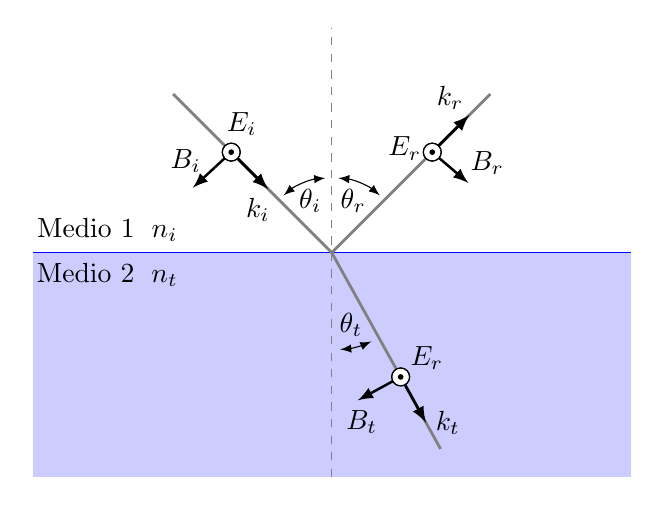
\begin{tikzpicture}[scale=.95]

%-------------------------------------------- Incidence media
\fill[blue!20] (-4,-3) rectangle (4,0);
% Interface
\draw[blue,line width=.5pt](-4,0)--(4,0); %%..5pt, interface]
% Vertical dashed line
\draw[dashed,gray,](0,-3)--(0,3);
% Media names
\node at (-3,.3) {Medio 1 $\; n_i$}; 
\node at (-3,-.3) {Medio 2 $\; n_t$};

%--------------------------------------------  Incident Wave
\draw[gray, line width=1pt](0:0cm)--(135:3cm);  % Light trajectory
\path (0,0)++(112.5:.75cm)node{$\theta_i$};       % Angle
\draw[latex-latex](95:1.cm)arc(95:130:1.cm);
 
    \draw[-latex,line width=1pt](135:1.9cm)--(135:1.2cm);    %Wave vector
    \path (0,0)++(141:0.9cm)node[left]{$\vb{k}_i$};     %Wave vector label
    
    \draw[-latex,line width=.9pt](135:1.9cm)--(155:2.05cm);  %B vector
    \path (0,0)++(148:2.3cm)node{$\vb{B}_i$}; 
    
    \path (0,0)++(125:2.1cm)node{$\vb{E}_i$};       % E vector
    
    \draw [fill= white](135:1.9cm)circle (0.12cm); % Vector perp. to surface
    \draw [black](135:1.9cm)circle (0.12cm);
    \filldraw[fill=black](135:1.9cm) circle(0.03cm); %%
    
%--------------------------------------------  Reflected Wave
\draw[gray,line width=1pt](0:0cm)--(45:3cm);  % Light trajectory
\path (0,0)++(67.5:.75cm)node{$\theta_r$};       % Angle
\draw[latex-latex](85:1.cm)arc(85:50:1.cm);
 
    \draw[-latex,line width=1pt](45:1.9cm)--(45:2.6cm);    %Wave vector
    \path (0,0)++(47.5:2.8cm)node[left]{$\vb{k}_r$};     %Wave vector label
    
    \draw[-latex,line width=.9pt](45:1.9cm)--(27:2.05cm);  %B vector
    \path (0,0)++(30:2.4cm)node{$\vb{B}_r$}; 
    
    \path (0,0)++(55:1.7cm)node{$\vb{E}_r$};       % E vector
    
    \draw [fill= white](45:1.9cm)circle (0.12cm); % Vector perp. to surface
    \draw [black](45:1.9cm)circle (0.12cm);
    \filldraw[fill=black](45:1.9cm) circle(0.03cm); %%

%--------------------------------------------  Transmitted Wave
\draw[gray,line width=1pt](0:0cm)--(-61:3cm);  % Light trajectory
\path (0,0)++(-75:1cm)node{$\theta_t$};       % Angle
\draw[latex-latex](-85:1.3cm)arc(-85:-66:1.3cm);
 
    \draw[-latex,line width=1pt](-61:1.9cm)--(-61:2.6cm);    %Wave vector
    \path (0,0)++(-61:2.6cm)node[right]{$\vb{k}_t$};     %Wave vector label

    \draw[-latex,line width=.9pt](-61:1.9cm)--(-80:2.005cm);  %B vector
    \path (0,0)++(-80:2.3cm)node{$\vb{B}_t$}; 
    
    \path (0,0)++(-48:1.9cm)node{$\vb{E}_r$};       % E vector
    
    \draw [fill= white](-61:1.9cm)circle (0.12cm); % Vector perp. to surface
    \draw [black](-61:1.9cm)circle (0.12cm);
    \filldraw[fill=black](-61:1.9cm) circle(0.03cm); %%     
 
\end{tikzpicture}
	\end{subfigure}
	\begin{subfigure}{.05\textwidth}\vspace{-4.5cm}\caption{}\label{sfig:Polp}	\end{subfigure}
	\begin{subfigure}{.43\textwidth}  \hspace*{-1cm}
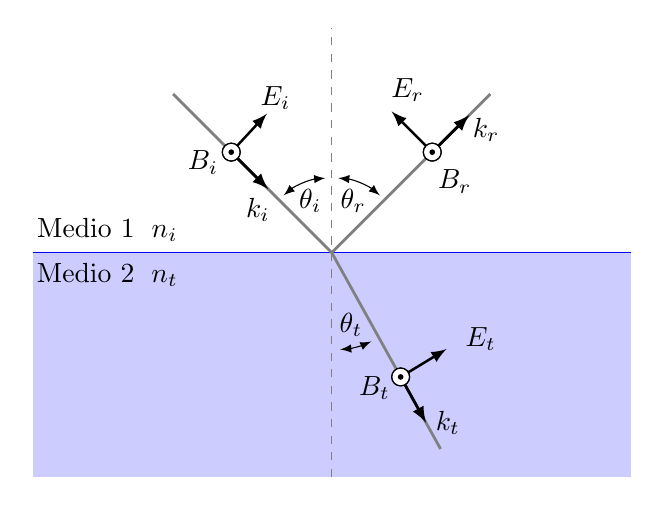
\begin{tikzpicture}[scale=.95]
%-------------------------------------------- Incidence media
\fill[blue!20] (-4,-3) rectangle (4,0);
% Interface
\draw[blue,line width=.5pt](-4,0)--(4,0); %%..5pt, interface]
% Vertical dashed line
\draw[dashed,gray,](0,-3)--(0,3);
% Media names
\node at (-3,.3) {Medio 1 $\; n_i$}; 
\node at (-3,-.3) {Medio 2 $\; n_t$};

%--------------------------------------------  Incident Wave
\draw[gray, line width=1pt](0:0cm)--(135:3cm);  % Light trajectory
\path (0,0)++(112.5:.75cm)node{$\theta_i$};       % Angle
\draw[latex-latex](95:1.cm)arc(95:130:1.cm);
 
    \draw[-latex,line width=1pt](135:1.9cm)--(135:1.2cm);    %Wave vector
    \path (0,0)++(141:0.9cm)node[left]{$\vb{k}_i$};     %Wave vector label
    
    \draw[-latex,line width=.9pt](135:1.9cm)--(115:2.05cm);  %E vector
    \path (0,0)++(110:2.2cm)node{$\vb{E}_i$}; 
%    \draw[-latex,line width=.9pt, red]((135:1.9cm)--(117:1.55cm); 

    
    \path (0,0)++(145:2.1cm)node{$\vb{B}_i$};       % B vector
    
    \draw [fill= white](135:1.9cm)circle (0.12cm);
    \draw [black](135:1.9cm)circle (0.12cm);
    \filldraw[fill=black](135:1.9cm) circle(0.03cm); %%    
    
    
%    \draw[line width=.6pt] (135:1.9cm)   % Esto esra paea hacer el vector salir de la hoja
%                         +(-135:.12cm) -- +(45:.12cm)
%                         +(-45:.12cm) -- +(135:.12cm);    
   
    
%--------------------------------------------  Reflected Wave
\draw[gray,line width=1pt](0:0cm)--(45:3cm);  % Light trajectory
\path (0,0)++(67.5:.75cm)node{$\theta_r$};       % Angle
\draw[latex-latex](85:1.cm)arc(85:50:1.cm);
 
    \draw[-latex,line width=1pt](45:1.9cm)--(45:2.6cm);    %Wave vector
    \path (0,0)++(43:2.4cm)node[right]{$\vb{k}_r$};     %Wave vector label
    
    \draw[-latex,line width=.9pt](45:1.9cm)--(67:2.05cm);  %E vector
    \path (0,0)++(65:2.4cm)node{$\vb{E}_r$};
  %  \draw[-latex,line width=.9pt, red](45:1.9cm)--(59:1.55cm); 
   % \draw[dashed,red,line width=.9pt](59:1.55cm)--(67:2.05cm);
    
    \path (0,0)++(30:1.9cm)node{$\vb{B}_r$};       % B vector
    
    \draw [fill= white](45:1.9cm)circle (0.12cm);
    \draw [black](45:1.9cm)circle (0.12cm);
    \filldraw[fill=black](45:1.9cm) circle(0.03cm); %%  


%--------------------------------------------  Transmitted Wave
\draw[gray,line width=1pt](0:0cm)--(-61:3cm);  % Light trajectory
\path (0,0)++(-75:1cm)node{$\theta_t$};       % Angle
\draw[latex-latex](-85:1.3cm)arc(-85:-66:1.3cm);
 
    \draw[-latex,line width=1pt](-61:1.9cm)--(-61:2.6cm);    %Wave vector
    \path (0,0)++(-61:2.6cm)node[right]{$\vb{k}_t$};     %Wave vector label
 
    \draw[-latex,line width=.9pt](-61:1.9cm)--(-40:2.005cm);  %E vector
%      \draw[-latex,line width=.9pt, red](-61:1.9cm)--(-45:2.3cm); 
    \path (0,0)++(-30:2.3cm)node{$\vb{E}_t$}; 
    
    \path (0,0)++(-72.5:1.9cm)node{$\vb{B}_t$};       % B vector
    
    \draw [fill= white](-61:1.9cm)circle (0.12cm);
    \draw [black](-61:1.9cm)circle (0.12cm);
    \filldraw[fill=black](-61:1.9cm) circle(0.03cm); %% 
\end{tikzpicture}
	\end{subfigure} 
	\caption{ Esquema de los campos EM para polarización \textbf{a)} \emph{s} y \textbf{b)} \emph{p} al cruzar una interfaz plana entre dos medios homogéneos, lineales e isótropos. Se considera que los campos EM mantienen la misma orientación antes y después de cruzar la interfaz.}	\label{fig:Polarizaciones}	
	\end{figure}	

La intensidad de una onda EM es proporcional al cuadrado de su amplitud. Por tanto, para calcular  la potencia  reflejada y transmitida se calculan primero los coeficientes de amplitud de reflexión $r$ y de transmisión $t$, que son el cociente del campo eléctrico reflejado, o transmitido, entre el campo incidente. Estos coeficientes son calculados empleando las condiciones a la frontera de los campos EMs [Ecs. \eqref{eqs:CFrontera}], por lo que el resultado depende de la polarización de la luz, es decir, de la dirección del campo eléctrico respecto al plano de incidencia (ver Fig. \ref{fig:Polarizaciones}). Para medios no magnéticos ($\tilde{\mu}=\mu_0$, cuando el campo eléctrico es perpendicular al plano de incidencia, como se muestra en la Fig. \ref{sfig:Pols}, se trata  de polarización \emph{s}, y los coeficientes de amplitud, en función del ángulo de incidencia, son 
	\begin{tcolorbox}[title = Coeficientes de amplitud para polarización \emph{s} ]
\vspace*{-1em}	\eqhalf{ r_s =
		\frac{\cos\theta_i-\sqrt{\left(\frac{n_t}{n_i}\right)^2-\sin ^2\theta_i}}
 			{\cos\theta_i + \sqrt{\left(\frac{n_t}{n_i}\right)^2-\sin ^2\theta_i}}, \label{eq:rs}}
	\eqhalf{ t_s =
		\frac{2\cos\theta_i}
 			{\cos\theta_i + \sqrt{\left(\frac{n_t}{n_i}\right)^2-\sin ^2\theta_i}.\label{eq:ts}}}
	\end{tcolorbox}	 \vspace*{-1em}\noindent
Si el campo eléctrico es paralelo al campo de incidencia, como en la Fig. \ref{sfig:Polp}, se trata de polarización \emph{p}, y los coeficientes de amplitud, en función del ángulo de incidencia, son 
	\begin{tcolorbox}[title = Coeficientes de amplitud para polarización \emph{p} ]
\vspace*{-1.5em}	\eqhalf{ r_p =
				 \frac{\left(\frac{n_t}{n_i}\right)^2 \cos\theta_i -
 				\sqrt{\left(\frac{n_t}{n_i}\right)^2-\sin^2\theta_i}}
 				{\left(\frac{n_t}{n_i}\right)^2 \cos \theta_i+
 				\sqrt{\left(\frac{n_t}{n_i}\right)^2-\sin^2\theta_i )}}, \label{eq:rp}}
	\eqhalf{ t_p =
				\frac{ 2 \left(\frac{n_t}{n_i}\right) \cos\theta_i}
 				{\left(\frac{n_t}{n_i}\right)^2 \cos \theta_i+
 				\sqrt{\left(\frac{n_t}{n_i}\right)^2-\sin^2\theta_i )}}.\label{eq:tp}}
	\end{tcolorbox}	 \vspace*{-1em}\noindent

Los coeficientes  de ampltiud dependen de las propiedades de los materiales, descritas por los índices de refracción presentes en sus expresiones, y según el valor de los índices de refracción se presentan distintos fenómenos físicos descritos por las Ecs. \eqref{eq:rs}--\eqref{eq:rp} . Si se comparan dos índices de refracción y uno de ellos es mayor que el otro, se dice que el material correspondiente al índice de refracción mayor posee una densidad óptica mayor. En el caso en el que la luz atraviesa una interfaz, entre dos medios lineales, homogéneos e isótropos, y el medio transmisión es  el más denso ópticamente, se dice que es incidencia externa y se se cumple la relación $n_t>n_i$. En caso contrario, es decir,  $n_t<n_i$ cuando  se trata de incidencia interna. Ambos casos son graficados en la Fig. \ref{fig:coefAmp} donde se presenta una interfaz de entre aire $n_{aire} = 1$ y vidio $n_{glass} = 1.5$.

\begin{figure}[b!]\centering
	\begin{subfigure}{.05\textwidth}\vspace{-4.75cm}\caption{}\label{sfig:coefExt}\end{subfigure}
	\begin{subfigure}{.43\textwidth} \hspace*{-1cm}
	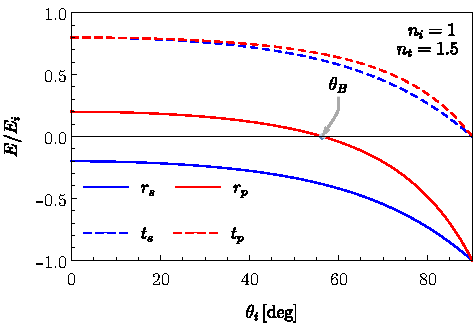
\includegraphics[scale=1,trim={00 00 00 00}, clip]{1-Teoria/figs/0-ampCoefExt}
	\end{subfigure}
	\begin{subfigure}{.05\textwidth}\vspace{-4.75cm}\caption{}\label{sfig:coefInt}\end{subfigure}
	\begin{subfigure}{.43\textwidth} \hspace*{-.9cm}
	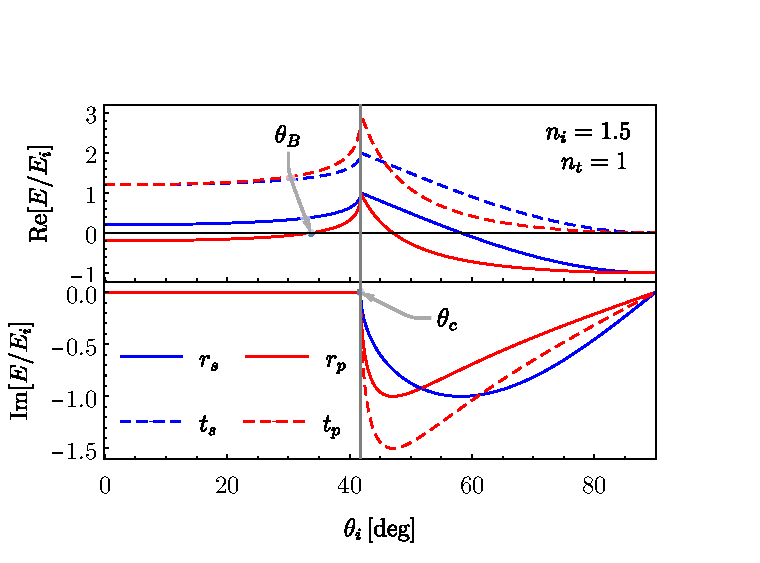
\includegraphics[scale=.7,trim={00 10 50 50 }, clip]{1-Teoria/figs/0-ampCoefInt}
	\end{subfigure}\vspace*{-.7em}
	\caption{ Coeficientes de amplitud, como función del ángulo de incidencia $\theta_i$, para polarización \textbf{a)} \emph{s} (en azul) y \textbf{b)} \emph{p (en rojo)}, para una interfaz entre vidrio ($n=1.5$) y aire ($n=1$).  Los coeficientes de amplitud de reflexión se representan mediante línea ssólidas; los de transmisión, mediante líneas punteadas.}	\label{fig:coefAmp}	
	\end{figure}	



Tanto para incidencia externa (Fig. \ref{sfig:coefExt}), así como para externa (Fig. \ref{sfig:coefExt}), el coeficiente de amplitud de reflexión para polarización \emph{p} $r_p$ [Ec. \eqref{eq:rp}] toma un valor nulo para un ángulo de incidencia. Éste es denominado ángulo de Brewster $\theta_B$, y cumple con la expresión
	\begin{equation}
	\tan\theta_B = \frac{n_t}{n_i}.
	\label{eq:Brewster}
	\end{equation}
Este comportamiento indica que para $\theta_i>\theta_B$, el campo eléctrico reflejado tiene una fase de $\pi$ radianes respecto al campo eléctrico incidente. De la Ec. \eqref{eq:Brewster} se deduce que el ángulo de Brewster de incidencia externa es complementaria al de incidencia interna.



Una característica que diferencia a la incidencia externa ($n_t<n_i$) de la externa ($n_t>n_i$) es el ángulo crítico $\theta_c$, sólo presente en incidencia interna, dado por
	\begin{equation}
	\sin\theta_c = \frac{n_t}{n_i}.
	\label{eq:Criticp}
	\end{equation}
Los coeficientes de amplitud [Ecs. \eqref{eq:rs}--\eqref{eq:tp}] para incidencia interna son cantidades reales para todo $\theta_i$ sin embargo, para incidencia externa sólo lo son para $\theta_i<\theta_c$. Para ángulos de incidencia mayors al crítico, los coeficientes de amplitud son cantidades complejas, lo que indica que los campos eléctricos incidente y reflejado tienen un desface, distinto de $\pi$, respecto al campo eléctrico incidente.
	

	\subsection{Reflectancia y transmitancia}

El análisis del comportamiento de las ondas EMs al cruzar una interfaz plana, entre dos medios lineales homogéneos e isótropos, en términos de las amplitudes de los campos eléctricos describen el comportamiento de la magnitud y los cambios de fase en los campos eléctricos  y no la cantidad de luz transmitida o reflejada. Esta información se obtiene de considerar la energía transportada por los campos EM, y por lo tanto se emplea el vector de Poynting [Ec. (\ref{eq:Poynting})], escrito únicamente en términos del campo eléctrico usando la relación $E = n B/c$
	\begin{equation}
	\vb{S} = n c\varepsilon_0 E_0^2 \vu{k}. \label{eq:PoyntingE}
	\end{equation}
Considerando campos eléctricos armónicos, es decir, tipo ondas planas, es necesario calcular el promedio temporal de la Ec. (\ref{eq:PoyntingE}). A este resultado se le denomina como irradiancia \cite{Hecht}
	\begin{equation}
	I = \langle S \rangle_t = \frac{nc\varepsilon_0}{2} E_0^2 \label{eq:Irr},
	\end{equation}
que es la energía promedio por unidad de tiempo, por unidad de área, transportada por los campos EMs en la dirección $\vu{k}$ \cite{griffiths2013electrodynamics}. Como se muestra en la fig. \ref{fig:areas}, las secciones transverasles de un haz de luz, definido por los campos eléctricos incidente, reflejado y transmitido, cambia en función de los ángulos de incidecia $\theta_i = \theta_r$, y del ángulo de transmisión $\theta_t$.




	\begin{figure}\centering
\begin{tikzpicture}[scale=.7]
%\draw (3.46,1.9) circle(2pt);ESTA ES LAREFERENCIA PARA ANTES DE MOVER LAS COSAS

%---------------------------------------------------------------------------------------- SUPERFICIE
\fill[blue!20]			
(-5,-1) -- (-3,2) 
-- (3,2) -- (5,-1)
--(-5,-1);						

\draw[dashed,gray](0,-4)--(0,5);  %---------------------------------------------------- Vertical dashed line

\node at (-4,-.5) {Medio 1 $\; n_i$}; %-------------------------------------------------- media names
\node at (-4,-1.5) {Medio 2 $\; n_t$};

%---------------------------------------------------------------------------------------- SPOT INTERFAZ
\fill[lgreen, opacity= .75] (0,.5) circle (2 and .6); 
\draw[black](0,.5) circle (2 and .6)		% -------------------------------------------  Etiqueta área
			(0,.5)node[]{$A$};	
%---------------------------------------------------------------------------------------- INCIDENTE
\path[shift = {(0,1.7)}] (0,0)++(112.5:1cm)node{$\theta_i$};   %------------------------- Angle
\draw[latex - latex,shift = {(0,2.1)}](-1,.5)arc(144.5:90:1.1cm);

\draw [-,shift = {(-2,.5)}, rotate = 55.5] (0,0) -- (0,3.2);   %------------------------- Cara del cilindro(Rota desde 90°)
\draw[-, shift = {(2,.5)},rotate = 55.5] (0,0) -- (0,6.3);

\draw[black, rotate = 50.75, shift = {(0,5)}](0,0) circle (1.145 and .3)		%-------- Tapa del cilidndro del del área
											  (1.1,.2)node[left]{ $A\cos\theta_i$};
\fill[lgreen, opacity= .5, rotate = 50.75, shift = {(0,5)}](0,0) circle (1.145 and .3);

%---------------------------------------------------------------------------------------- REFLEJADO
\path[shift = {(0,1.7)}] (0,0)++(67.5:1cm)node{$\theta_r$};   %------------------------- Angle
\draw[latex - latex ,shift = {(0,2.1)}](1,.5)arc(35:90:1.1cm);

\draw [-,shift = {(-2,.5)}, rotate = -55.5] (0,0) -- (0,6.3);   %------------------------- Cara del cilindro
\draw[-, shift = {(2,.5)},rotate = -55.5] (0,0) -- (0,3.2);

\draw[black, rotate = -50.75, shift = {(0,5)}](0,0) circle (1.145 and .3)		%-------- Tapa del cilidndro del del área
											  (-1.1,.2)node[right]{ $A\cos\theta_r$};
\fill[lgreen , opacity= .5, rotate = -50.75, shift = {(0,5)}](0,0) circle (1.145 and .3);

%---------------------------------------------------------------------------------------- TRANSMITIDO
\path[shift = {(.04,-2.6)}] (0,0)++(290:1)node{$\theta_t$};    %------------------------- Angle
\draw[latex - latex,shift = {(0,-3.25)}](0,0)arc(270:290:1.1cm);

\draw [-,shift = {(-2,.5)}, rotate = 33.5] (0,0) -- (0,-4.4);   %------------------------- Cara del cilindro
\draw[-, shift = {(2,.5)},rotate = 33.5] (0,0) -- (0,-2.5);

\draw[black, rotate = 29.2, shift = {(.5,-3)}](0,0) circle (1.675 and .3)		%-------- Tapa del cilidndro del del área
											  (1.675,.2)node[right]{ $A\cos\theta_t$};
\fill[lgreen, opacity= .5,  rotate = 29.2, shift = {(.5,-3)}](0,0) circle (1.675 and .3);

\end{tikzpicture}
	\caption{algo} \label{fig:hazcircular}
	\end{figure}


Considerando la irradiancia [Ec. (\ref{eq:Irr})] para cada una de las ondas en la interfaz en términos del área de la sección transversal del haz al llegar a la interfaz $A$ y los ángulos $\theta_i$ y $\theta_t$, la energía por unidad de tiempo transportada por cada haz es
	\begin{align*}
	P = I A \cos\theta = \frac{n c \varepsilon_0}{2} E_{0}^2 \cos\theta. 
	\end{align*}
Al normalizar la potencia reflejada, y la transmitida, respecto a la potencia del haz incidente.  se obtienen  la reflectancia $R$ y la transmitancia $T$, que al simplificar las expresiones se obtiene
	\begin{tcolorbox}[title = Reflectancia y transmitancia]
	\eqhalf{ R =  r r^*, \label{eq:R}}
	\eqhalf{ T = \frac{n_t\sin\theta_i}{n_i \sin\theta_t} t t^*.\label{eq:T}}
	\end{tcolorbox}	 \vspace*{-1em}\noindent	

	
\begin{figure}[t!]\centering
	\begin{subfigure}{.05\textwidth}\vspace{-4.75cm}\caption{}\label{sfig:frsnelExt}\end{subfigure}
	\begin{subfigure}{.43\textwidth} \hspace*{-1cm}
	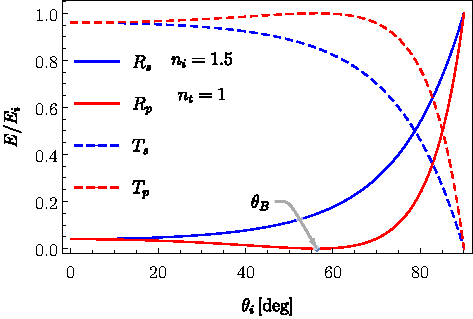
\includegraphics[scale=1,trim={00 00 00 00}, clip]{1-Teoria/figs/0-FrsnelExt}
	\end{subfigure}
	\begin{subfigure}{.05\textwidth}\vspace{-4.75cm}\caption{}\label{sfig:frsenlInt}\end{subfigure}
	\begin{subfigure}{.43\textwidth} \hspace*{-.9cm}
	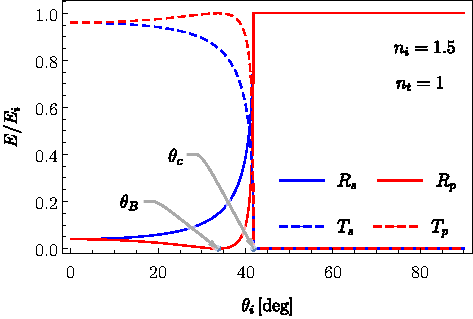
\includegraphics[scale=1,trim={00 00 00 00 }, clip]{1-Teoria/figs/0-FrsnelInt}
	\end{subfigure}\vspace*{-.7em}
	\caption{ Esquema de los campos EM para polarización \textbf{a)} \emph{s} y \textbf{b)} \emph{p} al cruzar una interfaz plana entre dos medios homogéneos, lineales e isótropos. Se considera que los campos EM mantienen la misma orientación antes y después de cruzar la interfaz.}	\label{fig:frsnel}	
	\end{figure}	

\section{Solución de Mie}

El problema de la absorción y el esparcimiento de luz por una partícula esférica fue resuelto por el físico alemán Gustav Mie en 1908 \cite{mie1908metallosung}. La solución de Mie consiste en la expansión de una onda plana, que ilumina una esfera, en una base esférica que cumple con las ecuaciones de Maxwell [Ecs. \eqref{eqs:Maxwell}],  y en las condiciones de continuidad que los campos EMs [Ecs. \eqref{eqs:CFrontera}] satisfacen en la superficie de la esfera \cite{bohren1998absorption,mie1908metallosung,horvath2009historic}. Existen publicaciones previas a la de Mie en donde el mismo enfoque es empleado \cite{horvath2009historic} sin embargo, en el trabajo de Mie se  desarrollan relaciones recursivas para la solución general, que facilitan el cálculo numérico, y se discute la convergencia de este resultado \cite{horvath2009historic}. Esto permitió que Mie expusiera diez casos prácticos, a diferencia de otros textos que se limitaban a pocos problemas experimentales \cite{horvath2009historic}.

Las ecuaciones de Maxwell, considerando una región del espacio sin cargas externas, y campos EMs armónicos en el tiempo, se reescriben como

	\begin{subequations}
	\eqhalf{\nabla\cdot \vb{E} = 0, }
	\eqhalf{\nabla\cdot \vb{H} = 0,}
	\eqhalf{\nabla \times \vb{E} = i\omega\tilde{\mu} \vb{H}, \label{seq:FLArm}}
	\eqhalf{\nabla\times\vb{H} = - i \omega\tilde{\varepsilon} \vb{E}, }	
	\label{eqs:MaxwellArm}
	\end{subequations} \vspace*{-1em}
	
\noindent	
en donde $\vb{H} = \vb{B}/\tilde{\mu}$ es el campo H, la permitividad eléctrica y la permeabilidad magnética del material son funciones continuas. Al desacoplar las ecuaciones de Maxwell, se concluye que los campos EMs son soluciones a la ecuación de Helmholz

	\begin{subequations}
	\eqhalf{\nabla^2 \vb{E}- k^2 \vb{E} = \vb{0},}
	\eqhalf{\nabla^2 \vb{H}- k^2 \vb{H} = \vb{0}.}
	\label{eq:Helmholtz}
	\end{subequations} \vspace*{-1em}
	
\noindent	
Para proceder con el cálculo de los campos EMs, se propone primero un campo vectorial $\vb{M}$ tal que
	\begin{align}
	\vb{M} &= \nabla \times \left(\vb{c} \psi\right),
	\label{eq:MrotCPsi}
	\end{align}
donde $\psi$ es una función escalar y $\vb{c}$ un vector \emph{constante} arbitrario; dado que $\vb{M}$ es el rotacional de  $\vb{c}\psi$, se cumple que $\nabla\cdot \vb{M} = \vb{0}$ y que $\vb{M}$ y $\vb{c}$ son vectores perpendiculares\footnote{Empleando la convención de la suma de Einstein y con $\epsilon_{ijk}$ el símbolo de  Levi-Civita: $M_i = [\nabla\times(\vb{c}\psi)]_i =  \epsilon_{ijk}\partial_jc_k\psi = -\epsilon_{jik}c_k\partial_j\psi = -\epsilon_{ikj}c_k\partial_j\psi  = - [\vb{c}\times\nabla\psi]_i$} . Empleando la Ec. \eqref{eq:MrotCPsi} para calcular la ecuación de Helmhotz para $\vb{M}$ se obtiene
	\begin{equation}
	\nabla^2 \vb{M} + k^2 \nabla\vb{M} = \nabla^2 \left[ \nabla\times\left(\vb{c} \psi\right) \right]+ 
			k^2 \nabla \times \left(\vb{c} \psi\right).\label{eq:HelmM1}
	\end{equation}
Dado que el operador laplaciano y el rotacional conmutan\footnote{ Para un campo vectorial arbitrario $\vb{A}$ se cumple que $\nabla^2\vb{A} = \nabla(\nabla\cdot\vb{A}) - \nabla\times(\nabla\times\vb{A})$, por lo que el rotacional del laplaciano de $\vb{A}$ es $ \nabla\times( \nabla^2\vb{A})=\nabla\times[\nabla(\nabla\cdot\vb{A})  ]-  \nabla\times[\nabla\times(\nabla\times \vb{A})] = -  \nabla\times[\nabla\times(\nabla\times \vb{A})] $ pues el rotacional del gradiente de cualquier función es nulo. Además, al sustituir $\vb{A}\to \nabla\times\vb{A}$ en la expresión del laplaciano de $\vb{A}$ y  considerando que la divergencia del rotacional de cualquier función es nulo, se obtiene que$ \nabla^2(\nabla\times\vb{A})=\nabla[\nabla\cdot(\nabla\times\vb{A})  ]-  \nabla\times[\nabla\times(\nabla\times \vb{A})] = -  \nabla\times[\nabla\times(\nabla\times \vb{A})] $. Por tanto, $\nabla^2$ y $\nabla\times$ con operadores que conmutan.}, la Ec. \eqref{eq:HelmM1} puede reescribirse como
	\begin{equation}
	\nabla^2 \vb{M} + k^2 \nabla\vb{M}  = \nabla\times\left[\vb{c}\left( \nabla^2\psi+k^2\psi \right) \right].
	\end{equation}
	
Se define también el vector $\vb{N}$ dado por la expresión
	\begin{equation}
	\vb{N} = \frac{\nabla\times \vb{M}}{k}, \label{eq:NrotM/k}
	\end{equation}
cuyo laplaciano es $\nabla^2 \vb{N} = \nabla^2( \nabla\times \vb{M} /k) =  \nabla\times (\nabla^2\vb{M} /k) $, pues el rotacional y el laplaciano son operadores que conmutan entre sí. Por tanto, la ecuación de Helmholtz para $\vb{N}$ es
	\begin{align}
	\nabla^2 \vb{N} + k^2 \vb{N} =  \nabla\times \left( \frac{\nabla^2 \vb{M}}{k} \right) + k \nabla\times \vb{M} 
		 = \frac{1}{k} \nabla\times \left( \nabla^2 \vb{M} + k^2  \vb{M} \right).
	\end{align}

Los campos $\vb{M}$ y $\vb{N}$ cumplen con la Ec. de la ecuación de Helmholtz vectorial [Ec. \eqref{eq:Helmholtz}] si, y sólo si, la función escalar $\psi$ cumple con la ecuación de Helmholtz escalar $\nabla^2 \psi + k^2 \psi = 0$. Si este es el caso, entonces, el rotacional de $\vb{N}$ está dado por
	\begin{align}
	\nabla\times \vb{N} &= \nabla\times \qty(\frac{\nabla\times \vb{M}}{k})  
						= \frac{\nabla\qty(\nabla\cdot\vb{M})-\nabla^2\vb{M}}{k}
						= - \frac{\nabla^2 \vb{M}}{k}
						= \frac{k^2 \vb{M}}{k}
						= k \vb{M}.\label{eq:rotN}
	\end{align}
	
Los campos vectoriales $\vb{M}$ y $\vb{N}$ son conocidos como los \emph{armónicos  vectoriales}, $\psi$ como su función generadora y $\vb{c}$ como el vector de guía o vector piloto. Los armónicos esféricos vectoriales $\vb{M}$ y $\vb{N}$  cumplen con tener divergencia nula y que el rotacional de uno es porporcional al otro [Ecs. \eqref{eq:NrotM/k} y \eqref{eq:rotN}], es decir, que cumplen con las ecuaciones de Maxwell y con la ecuación de Helmholtz ---por lo que cuentan con las caraterísticas de campos EMs--- siempre que se cumpla que
	\begin{tcolorbox}[title = $\mathbf{\psi}$: Función generadora de los armónicos  vectoriales, ams align ]
	\nabla^2 \psi + k^2 \psi  = 0.\label{eq:AV_psi}
	\end{tcolorbox}

	\subsection{Solución a la ecuación de onda con simetría esférica}


Para poder encontrar las soluciones del campo esparcido por una esfera basta entonces con encontrar las soluciones de la Ec. \eqref{eq:AV_psi} con la geometría deseada e imponer las condiciones a la frontera de los campos EMs. Suponiendo una partícula esférica, se escoge el vector piloto $\vb{c}$ como $\vb{r}$ (ver Fig. \ref{fig:EsferaA}), por lo que $\vb{M}$ es solución a la ecuación de Helmholtz en coordenadas esféricas $(r,\theta, \varphi)$, además de que se cumple que $\vb{M}$ será tangencial a cualquier esfera de radio $r=\norm{\vb{r}}$ constante.

	\begin{figure}[h!]\centering
	\begin{minipage}[c]{.95\linewidth}\centering
	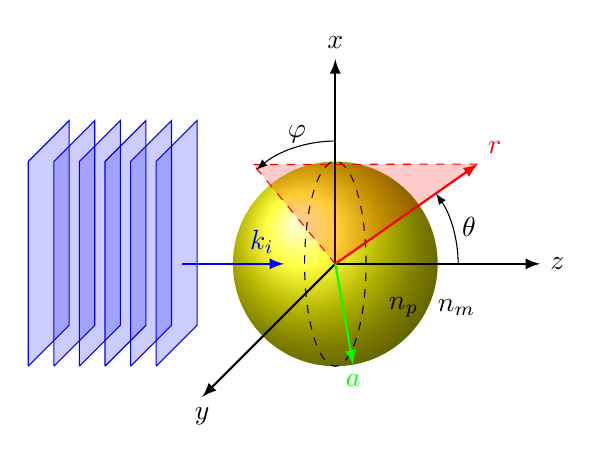
\begin{tikzpicture}[scale=1.3]

\coordinate (O) at (0,0);

%------------------------------------------------------- Particle
\shade[ball color=yellow, opacity = 1] (O) circle (1); 
\draw[dashed] (O) ellipse (.3 and 1);

%------------------------------------------------------- Coordinate system axes
\draw[- latex, thick] (O) -- (-1.3,-1.3) node[anchor=north ]{$y$};
\draw[- latex, thick] (O) -- (2,0) node[anchor= west]{$z$};
\draw[- latex, thick] (O) -- (0,2) node[anchor=south]{$x$};


%------------------------------------------------------- Vector \vb{r}
\draw[thick,red,- latex] (O) -- (35:1.7) node[anchor=south west]{$\vb{r}$}; 
\draw[-, dashed,red] (O) -- (-.8,.97);		%xy proyection
\draw[-,dashed,red] (-.8,.97) -- (35:1.7) ;	%normal proyection
\fill[red,opacity=.2] (O)-- (-.8,.97)--(35:1.7)--(O);  %Shade
	
	
%------------------------------------------------------- polar variables	
\path (O)++(35/2:1.2)node[anchor=west]{$\theta$};    
\draw[- latex](0:1.2)arc(0:35:1.2);

\path (O)++(100:1.1)node[anchor=south east]{$\varphi$};    
\draw[- latex](90:1.2)arc(90:130:1.2);
	

%------------------------------------------------------- Particule radius & n	
\draw[thick,green,- latex] (O) -- (-80:1) node[anchor=north]{$\vb{a}$};  

\path (O)++(-25:1) node[anchor=east]{$n_p$};
\path (O)++(-25:1) node[anchor=west]{$n_m$};


%------------------------------------------------------- Plane wave

\def\dx{1.75}
\def\dy{1}
\def\dr{.4}

\foreach \i in {-5,...,-1,0}{
	\fill[opacity=.2,blue] (\i*.25-\dx,-\dy)--(\i*.25-\dx,\dy)--
							(\i*.25-\dx+\dr, \dy+\dr)--(\i*.25-\dx+\dr, -\dy+\dr);
	\draw[blue] (\i*.25-\dx,-\dy)--(\i*.25-\dx,\dy)--
							(\i*.25-\dx+\dr, \dy+\dr)--(\i*.25-\dx+\dr, -\dy+\dr)--
							(\i*.25-\dx,-\dy);}									

\draw[- latex,thick,blue] (-1.5,0)--(-1.5+1,0) node[anchor=south east]{$\vb{k}_i$};

	
\end{tikzpicture}
		\caption{ Esfera de radio $a$ e ínidce de refracción $n_p$, inmersa en una matriz con índice $n_m$. La esfera es iluminada por una onda plana de luz con vector de onda $\vb{k}_i$ que viaja en la dirección $\hat{e}_z$.}\label{fig:EsferaA}
	\end{minipage}
	\end{figure}
	
En coordenadas esféricas la Ec. \eqref{eq:AV_psi} es
	\begin{equation}
	\frac{1}{r^2} \pdv{r}\qty(r^2\pdv{\psi}{r})+ 
	\frac{1}{r^2\sin\theta}\pdv{\theta}\qty(\sin\theta\pdv{\psi}{\theta})
	 + \frac{1}{r^2\sin^2\theta}\pdv[2]{\psi}{\varphi} + k^2 \psi =0. \label{eq:AEV_psi}
	\end{equation}
Para resolver la Ec. \eqref{eq:AEV_psi} se asume que $\psi$ es el producto de tres funciones y cada una de éstas depende únicamente en una variable, es decir,
	\begin{equation}
	\psi (r,\theta, \varphi) = R(r)\Theta(\theta) \Phi(\varphi). \label{eq:psiEsf}
	\end{equation}
La resolución de la Ec. \eqref{eq:AV_psi} busca construir un conjunto de funciones linealmente independientes que sean una base para los campos EMs incidentes, esparcidos y dentro de la esfera. Al sustituir la Ec. \eqref{eq:psiEsf} en la Ec. \eqref{eq:AEV_psi},  y multiplicar por $r^2/R\Theta\Phi$ y despejando los términos que dependen únicamente de $r$, se obtiene como resultado que una función con dependencia radial es igual a una función con dependencia angular, por lo tanto se igualan a una constante $\ell (\ell +1)$, es decir
	\begin{equation}
\mathrlap{\overbrace{\phantom{\frac{1}{R} \dv{r}\qty(r^2\dv{R}{r})+  k^2 r^2 = \ell (\ell +1)}}^{\text{radial}}}
									\frac{1}{R} \dv{r}\qty(r^2\dv{R}{r})+  k^2 r^2 = 
      \mathrlap{\underbrace{\phantom{\ell (\ell +1)=
									-\frac{1}{\Theta\sin\theta}\dv{\theta}\qty(\sin\theta\dv{\Theta}{\theta})
								  \frac{1}{\sin^2\theta}\frac{1}{\Phi}\pdv[2]{\psi}{\varphi} }}_{\text{angular}}}
						 \ell (\ell +1)=
						-\frac{1}{\Theta\sin\theta}\dv{\theta}\qty(\sin\theta\dv{\Theta}{\theta})
					 - \frac{1}{\sin^2\theta}\frac{1}{\Phi}\pdv[2]{\psi}{\varphi}.\label{eq:radAng}
	\end{equation}
Si la parte angular de la Ec. \eqref{eq:radAng} se multiplica por $\sin^2\theta$, y se despejan los términos que dependen de $\theta$, se obtiene que una función que depende únicamente de $\theta$ es igual a una que depende únicamente de $\varphi$, por lo que ambas partes se igualan a la constante $m^2$. Tanto $\ell$ en la Ec. \eqref{eq:radAng}, como $m$ son constantes que se determinan ante condiciones impuestas a $\psi$. Tras este procedimiento ---llamado separación de variables--- se tiene entonces que las funciones $R(r),\, \Theta(\theta), \mbox{ y } \Phi(\varphi)$ cumplen con las ecuaciones
\begin{align}
\frac{1}{\Phi}\pdv[2]{\psi}{\varphi} &+ m^2 \Phi =0. \label{eq:Phi}\\
\frac{1}{\sin\theta}\dv{\theta}\qty(\sin\theta\dv{\Theta}{\theta}) &+ \qty[\ell(\ell+1)- \frac{m^2}{\sin^2\theta}]\Theta =0,\label{eq:Theta}\\
\dv{r}\qty(r^2\dv{R}{r}) &+ \qty[ k^2 r^2 - \ell (\ell +1)] R =0. \label{eq:R}
\end{align}

Dado que $\psi$ debe ser una función con periodicidad $2\pi$ en $\varphi$, es decir que $\psi(\varphi) = \psi(\varphi+2\pi)$, las soluciones linealmente independientes de la Ec. \eqref{eq:Phi} son

	\begin{subequations}
	\eqhalf{\Phi_e(\varphi) = \cos(m\varphi),}
	\eqhalf{\Phi_o(\varphi) = \sin(m\varphi),} 
	\end{subequations}
	
\noindent	
con $m$ un número entero no negativo. Los subíndices $e$ y $o$ hacen referencia a que son funciones pares e impares respectivamente.

Haciendo el cambio de variable $\mu = \cos\theta$ en la Ec. \eqref{eq:Theta} , ésta se reescribe como
	\begin{equation*}
	\qty(1-\mu^2) \dv[2]{\Theta}{\mu} - 2 \mu \dv{\Theta}{\mu} + \qty[\ell(\ell+1)-\frac{m^2}{(1-\mu^2)}]\Theta= 0,
	\end{equation*}
cuyas soluciones que cumplen con ser finitas en $\theta = 0$ y $\theta = \pi$ ---o bien $\mu=\pm1$--- imponen que $\ell = m, m+1,m+2,\ldots$. Las soluciones a la Ec. \eqref{eq:Theta} son entonces las \emph{funciones asociadas de Legendre} $P_\ell^m(\cos\theta)$ de grado $\ell$ y orden $m$, las cuales se reducen a los polinomios de Legendre $P_\ell(\cos\theta)$ cuando $m=0$. Las funciones asociadas de Legendre son ortogonales, obedeciendo la relación
	\begin{equation}
	\int_{-1}^1P_\ell^m(\mu) P_{\ell'}^md\mu = \delta_{\ell,\ell'}\frac{2}{2\ell+1}\frac{(\ell+m)!}{(\ell-m)!},
	\label{eq:ortLegendre}
	\end{equation}
donde $\delta_{\ell,\ell'}$ es la delta de Kronecker y $\mu=\cos\theta$. Asimismo, las funciones asociadas de Legendre se relacionan con los polinomios de Legendre mediante la identidad
	\begin{equation}
	P_\ell^m (\mu) = (1-\mu^2)^{m/2}\dv[m]{P_\ell(\mu)}{\mu},
	\label{eq:FAL-PL}
	\end{equation}
de donde se obtiene que $\eval{P_\ell^m(\cos\theta)}_{\theta=0,\pi}=0$ para toda $m$ distinta de cero. %Asimismo, de la Ec. \eqref{eq:FAL-PL} se obtiene que para $m=1$ se cumple que
%	\begin{equation}
%	P_\ell^1(\cos\theta) = - \dv{P_\ell}{\theta} (\cos\theta ).
%	\label{eq:FALm=1}
%	\end{equation}
%Además, los polinomios de Legendre cumplen con la relación de recuerrencia
%	\begin{equation}
%	\dv{\theta}\qty[\sin\theta \dv{P_\ell}{\theta} ( \cos \theta ) ] = -\ell(\ell+1)\sin\theta P_\ell( \cos\theta )
%	\label{eq:PolLegeRec}
%	\end{equation}

Para resolver la Ec. \eqref{eq:R} se emplea el cambio de variable $\rho = k r$ y de define la función $Z =R\sqrt{\rho}$, por lo que la Ec. \eqref{eq:R} se reescribe como
	\begin{equation}
	\rho \dv{\rho}\qty(\rho\dv{Z}{\rho})+\qty[\rho^2-\qty(\ell+\frac12)^2] Z = 0,
	\end{equation}
cuyas soluciones son las \emph{funciones esféricas de Bessel} $j_\ell$ y $y_\ell$ o cualquier combinación lineal de ellas. Por simplificación en futuros cálculos, se toman como soluciones de la Ec. \eqref{eq:R} las funciones

	\begin{subequations}
	\eqhalf{j_\ell (\rho) = \sqrt{\frac{\pi}{2\rho}} J_{\ell+1/2}(\rho), \label{eq:jn}}
	\eqhalf{y_\ell (\rho) = \sqrt{\frac{\pi}{2\rho}} Y_{\ell+1/2}(\rho), \label{eq:yn}}
	\eqhalf{h_\ell^{(1)} (\rho) = j_\ell(\rho) + i y_\ell(\rho), \label{eq:h1}}
	\eqhalf{h_\ell^{(2)} (\rho) =  j_\ell(\rho) - i y_\ell(\rho), \label{eq:h2}}
	\label{eqs:SphBessel}
	\end{subequations}

\noindent	
en donde $J_\ell$ y $Y_\ell$ son las \emph{funciones de Bessel del primer y segundo tipo} respectivamente y $h_\ell$ son las \emph{funciones esféricas de Bessel del tercer tipo}, también denominadas como \emph{funciones esféricas de Hankel}. Todas las funciones esféricas de Bessel $z_\ell$ ---donde $z_\ell$ es cualquier función de las Ecs. \eqref{eqs:SphBessel}--- cumplen con las  relaciones de recurrencia
	\begin{align}
	z_{\ell-1}(\rho) + z_{\ell+1}(\rho) &=\frac{2\ell+1}{\rho} z_\ell(\rho),\\
	(2\ell + 1) \dv{z_\ell(\rho)}{\rho} &= \ell z_{\ell-1}(\rho) - (\ell+1)z_{\ell+1}(\rho),
	\end{align}
en donde los primeros dos órdenes ($\ell=0,1$) de $j_\ell$ y $y_\ell$ son

	\eqhalf{j_0(\rho) = \frac{\sin\rho}{\rho}, \notag}
	\eqhalf{j_1(\rho) = \frac{\sin\rho}{\rho^2}-\frac{\cos\rho}{\rho},\notag}
	\eqhalf{y_0(\rho) = -\frac{\cos\rho}{\rho},\notag}
	\eqhalf{y_1(\rho) = -\frac{\cos\rho}{\rho^2}-\frac{\sin\rho}{\rho}.\notag}

\vspace*{-1em}\noindent
Por tanto, las funciones generadoras de los armónicos esféricos vectoriales son

	\begin{subequations}
	\eqhalf{\psi_{em\ell} = \cos(m\varphi) P_\ell^m( \cos \theta) z_\ell(k r),}
	\eqhalf{\psi_{om\ell} = \sin(m\varphi) P_\ell^m( \cos \theta) z_\ell(k r),}
	\label{eq:psieo}
	\end{subequations}
	
\noindent	
por lo que se construyen cuatro armónicos esféricos vectoriales. Empleando las Ecs. \eqref{eq:psieo} en la Ec. \eqref{eq:MrotCPsi}, con $\vb{r}$ como el vector piloto, se obtiene como resultado $\vb{M}_{em\ell}$ y $\vb{M}_{om\ell}$, dados por las expresiones
	\begin{subequations}
	\begin{tcolorbox}[title = Armónicos esféricos vectoriales $\vb{M}_{em\ell}$ y $\vb{M}_{om\ell}$, ams align ]
	\vb{M}_{em\ell} = &-m\sin(m\varphi)z_\ell(kr) \frac{P_\ell^m(\cos\theta)}{\sin\theta} \vu{e}_\theta
					-\cos(m\theta)z_\ell(kr) \dv{P_\ell^m(\cos\theta)}{\theta}(\cos\theta) \vu{e}_\varphi,\label{seq:Meml} \\
	\vb{M}_{om\ell} = & m\cos(m\varphi)z_\ell(kr) \frac{P_\ell^m(\cos\theta)}{\sin\theta} \vu{e}_\theta
					-\sin(m\theta)z_\ell(kr) \dv{P_\ell^m(\cos\theta)}{\theta}(\cos\theta) \vu{e}_\varphi.	\label{seq:Moml}				
	\end{tcolorbox}
	
Para el cálculo $\vb{N}_{em\ell}$ y $\vb{N}_{om\ell}$ se sustituyen las Ecs. \eqref{seq:Meml} y \eqref{seq:Moml} en la Ec. \eqref{eq:NrotM/k}. Para simplificar las expresiones de las componentes radiales de  $\vb{N}_{em\ell}$ y $\vb{N}_{om\ell}$, se agrupan los términos que dependen de $\varphi$ y $kr$ y, dado que las funciones asociadas de Legendre cumplen con la relación 
\begin{equation*}
-\ell(\ell+1) P_\ell^m (\cos\theta)= \frac{1}{\sin\theta}\dv{\theta}\qty(\sin\theta\dv{P_\ell^m(\cos\theta)}{\theta}) - \frac{m^2}{\sin^2\theta}P_\ell^m(\cos\theta),
\end{equation*}
que es una consecuencia de la Ec. \eqref{eq:Theta}, las expresiones de $\vb{N}_{em\ell}$ y $\vb{N}_{om\ell}$ son
	\begin{tcolorbox}[title = Armónicos esféricos vectoriales $\vb{N}_{em\ell}$ y $\vb{N}_{om\ell}$, ams align, breakable ]
	\vb{N}_{em\ell} =&\cos(m\varphi) \frac{z_\ell(kr)}{kr} \ell(\ell+1)P_\ell^m(\cos\theta) \vu{e}_r \notag\\
	&+ \cos(m\varphi)  \frac{1}{kr} \dv{(kr)}\qty\Big[kr\, z_\ell(kr)] \dv{P_\ell^m(\cos\theta)}{\theta}(\cos\theta) \vu{e}_\theta
	 \label{seq:Neml} \\
		&- m \sin(m\varphi) \frac{1}{kr} \dv{(kr)}\qty\Big[kr\, z_\ell(kr)] \frac{P_\ell^m(\cos\theta)}{\sin\theta}
		 \vu{e}_\varphi, \notag\\			
	\vb{N}_{om\ell} =&\sin(m\varphi) \frac{z_\ell(kr)}{kr} \ell(\ell+1)P_\ell^m(\cos\theta) \vu{e}_r \notag\\
	&+ \sin(m\varphi)  \frac{1}{kr} \dv{(kr)}\qty\Big[kr\, z_\ell(kr)] \dv{P_\ell^m(\cos\theta)}{\theta}(\cos\theta) \vu{e}_\theta
	 \label{seq:Noml} \\
		&+ m \cos(m\varphi) \frac{1}{kr} \dv{(kr)}\qty\Big[kr\, z_\ell(kr)] \frac{P_\ell^m(\cos\theta)}{\sin\theta}
		 \vu{e}_\varphi. \notag							
	\end{tcolorbox}\label{eq:AEV}
	\end{subequations}

Los armónicos esféricos vectoriales son solución a la ecuación de Helmholtz, por lo que cualquier solución de campo EM puede escribirse como una serie infinta en términos de las Ecs. \eqref{eq:AEV}. Para resolver el problema de los campos EMs esparcidos por una partícula esférica, se expande una onda plana $\vb{E}^i$ en la base de los armónicos esféricos vectoriales. Para esto, se emplean sus  condiciones de ortogonalidad.

Las funciones $\sin(m\varphi)$ y $\cos(m\varphi)$ obedecen las relaciones de ortogonalidad
 	\begin{subequations}
	\begin{align}
	\int_0^{2\pi} \sin(m\varphi) &\cos(m' \varphi) \dd\varphi = 0 \qquad \forall\, m,m',\label{seq:ortSinCos}\\
	\int_0^{2\pi} \sin(m\varphi) \sin(m'\varphi)\dd\varphi &=  \int_0^{2\pi} \cos(m\varphi) \cos(m'\varphi)\dd\varphi  = \delta_{m,m'}\frac{\pi}{2}.\label{seq:ortCos2}
	\end{align}\label{eq:SinCos}
 	\end{subequations}
Por la Ec. \eqref{seq:ortSinCos} se cumple que el producto interior\footnote{Se define el producto interior $\langle \vb{A},\vb{B} \rangle_{\theta,\varphi}$ como $\langle \vb{A},\vb{B} \rangle_{\theta,\varphi} \equiv \int_0^{2\pi}\int_0^\pi \vb{A}\cdot\vb{B} \sin\theta \dd\theta \dd\varphi$} entre $\vb{M}_{em\ell}$ y $\vb{M}_{om'\ell'}$, y $\vb{N}_{em\ell}$ y $\vb{N}_{om'\ell'}$ es
	\begin{tcolorbox}[ ams align ]
		\langle\vb{M}_{em\ell}, \vb{M}_{om'\ell'} \rangle_{\theta,\varphi} =
		\langle\vb{N}_{em\ell}, \vb{N}_{om'\ell'} \rangle_{\theta,\varphi} = 0
		&\qquad \forall\,  m,m',\ell, \ell',\\
		\intertext{así como también}
		\langle\vb{M}_{om\ell}, \vb{N}_{em'\ell'} \rangle_{\theta,\varphi} = 
		\langle\vb{M}_{om\ell}, \vb{N}_{om'\ell'} \rangle_{\theta,\varphi} = 	
		\langle\vb{M}_{em\ell}, \vb{N}_{em'\ell'} \rangle_{\theta,\varphi} = 	0
		&\qquad \forall\,  m,m',\ell, \ell'.				
	\end{tcolorbox}\noindent
pues $\vb{M}$ tiene componente nula en $\vu{e}_r$ y en los demás términos se encuentra la Ec. \eqref{seq:ortSinCos}. Las Ecs. \eqref{eq:SinCos} implican que todos los armónicos esféricos vectoriales orden $m$ distinto  son ortogonales entre sí.\\

 El producto interior entre $\vb{M}_{em\ell}$ y $\vb{N}_{om\ell'}$, empleando el resultado de la Ec. \eqref{seq:ortCos2} con $m=m'$, está dado por
	\begin{align}
		\langle\vb{M}_{em\ell},  \vb{N}_{om\ell'} \rangle_{\theta,\varphi} &= - \frac{\pi}{2} \frac{z_\ell (\rho)}{\rho}\dv{z_{\ell'}(\rho)}{\rho}	m
							 \int_0^\pi\qty[P_\ell^m(\cos \theta )\dv{P_{\ell'}^m(\cos \theta )}{\theta}+ 
							  \dv{P_{\ell}^m(\cos \theta )}{\theta}P_{\ell'}^m(\cos \theta )] \dd\theta \notag\\
					 &=- \frac{\pi}{2} \frac{z_\ell (\rho)}{\rho}\dv{z_{\ell'}(\rho)}{\rho}	m 
					 	\int_0^\pi \dv{\theta}\qty[P_\ell^m(\cos\theta)P_{\ell'}^m(\cos\theta)]\dd\theta \notag\\
					 &=- \frac{\pi}{2} \frac{z_\ell (\rho)}{\rho}\dv{z_{\ell'}(\rho)}{\rho}	m \eval{P_\ell^m(\cos\theta)P_{\ell'}^m(\cos\theta)}_0^\pi.
					 	\label{eq:MeNo}
	\end{align}
Mediante un procedimiento semejante se obtiene que $\langle\vb{M}_{em\ell},  \vb{N}_{om\ell'} \rangle_{\theta,\varphi}=\langle\vb{M}_{om\ell},  \vb{N}_{em\ell'} \rangle_{\theta,\varphi}$. Haciendo uso de la relación entre las funciones asociadas de Legndre con los polinomios de Legendre [Ec. \eqref{eq:FAL-PL}] se obtiene que $P_\ell^m(\cos\theta)=0$ para $\theta=0,\pi$ y $m\neq 0$. Sin embargo, si en la Ec. \eqref{eq:MeNo} $m$ es igual a cero, el producto interior también es nulo, por lo que se cumple que 
	\begin{tcolorbox}[ ams align ]
		\langle\vb{M}_{em\ell},  \vb{N}_{om\ell'} \rangle_{\theta,\varphi}=
		\langle\vb{M}_{om\ell},  \vb{N}_{em\ell'} \rangle_{\theta,\varphi}= 0	
		\qquad \forall\, \ell, \ell'\, m.
	\end{tcolorbox}
Las expresiones del  producto interior entre $\vb{M}_{em\ell}$ y $\vb{M}_{em\ell'}$, y $\vb{N}_{em\ell}$ y $\vb{N}_{em\ell'}$, empleando el resultado de la Ec. \eqref{seq:ortCos2} con $m=m'$, y la relación de ortogonalidad de las funciones asociadas de Legendre [Ec. \eqref{eq:ortLegendre}] son
	\begin{align*}
		\langle\vb{M}_{em\ell},  \vb{M}_{em\ell'} \rangle_{\theta,\varphi} =& 
				\frac{\pi}{2} z_\ell (\rho) z_{\ell'}(\rho)\times	 \int_0^\pi\qty[\frac{m^2}{\sin^2\theta}P_\ell^m(\cos\theta)P_{\ell'}^m(\cos\theta)
				 +\dv{P_\ell^m(\cos\theta)}{\theta}\dv{P_{\ell'}^m(\cos\theta)}{\theta}]\sin\theta\dd\theta\\
		\langle\vb{N}_{em\ell},  \vb{N}_{em\ell'} \rangle_{\theta,\varphi} =&
				\frac{\pi}{2} \qty[\frac{z_\ell(\rho)}{\rho}\ell(\ell+1)]^2\frac{2}{2\ell+1}\frac{(\ell+m)!}{(\ell-m)!}\delta_\ell^{\ell'}+
				\frac{\pi}{2} \frac{1}{\rho^2}\dv{\rho}\qty[\rho z_\ell (\rho)]\dv{\rho}\qty[\rho z_{\ell'}(\rho)]\\
				&\times \int_0^\pi\qty[\frac{m^2}{\sin^2\theta}P_\ell^m(\cos\theta)P_{\ell'}^m(\cos\theta)
					+\dv{P_\ell^m(\cos\theta)}{\theta}\dv{P_{\ell'}^m(\cos\theta)}{\theta}]\sin\theta\dd\theta.				 
	\end{align*}
Asimismo, se cumple que  $\langle\vb{M}_{em\ell},  \vb{M}_{em\ell'} \rangle_{\theta,\varphi}=\langle\vb{M}_{om\ell},  \vb{M}_{om\ell'} \rangle_{\theta,\varphi}$ y $\langle\vb{N}_{em\ell},  \vb{N}_{em\ell'} \rangle_{\theta,\varphi}=\langle\vb{N}_{om\ell},  \vb{N}_{om\ell'} \rangle_{\theta,\varphi}$. Sustituyendo $P_\ell^m(\cos\theta)$ en la Ec. \eqref{eq:Theta} y multiplicándola por $P_{\ell'}^m(\cos\theta)$, operando de la misma forma intercambiando los papeles de $P_\ell^m(\cos\theta)$  y $P_{\ell'}^m(\cos\theta)$ y sumando ambos resultados se llega a la expresión 
	\begin{align}
	2\frac{m^2}{\sin^2\theta}P_\ell^m P_{\ell'}^m \sin\theta =&
					 P_\ell\dv{\theta}\qty[\sin\theta \dv{P_{\ell'}^m}{\theta}] P_{\ell'}\dv{\theta}\qty[\sin\theta \dv{P_\ell^m}{\theta}]
					 +	\ell(\ell+1)P_\ell^m P_{\ell'}^m	 \sin\theta  \notag\\
					 &+ \ell'(\ell'+1)P_\ell^m P_{\ell'}^m\sin\theta, \label{eq:PnPn'}
	\end{align}
en donde se obvia el argumento $\cos\theta$. Dado que 
	\begin{equation*}
	\dv{\theta}\qty[P_{\ell'}^m\sin\theta  \dv{P_\ell^m}{\theta}] 
	= P_{\ell'}^m\dv{\theta}\qty[\sin\theta \dv{P_\ell^m}{\theta}] + \sin\theta\dv{P_{\ell'}^m}{\theta}\dv{P_\ell^m}{\theta},
	\end{equation*}
sumando $2\sin\theta\dd P_{\ell'}^m\dd\theta \dd P_\ell^m \dd\theta$ de ambos lados de la Ec. \eqref{eq:PnPn'} y agrupando términos, se obtiene que el integrando presente en los productos interiores de  $\vb{M}_{em\ell}$ y $\vb{M}_{em\ell'}$, y $\vb{N}_{em\ell}$ y $\vb{N}_{em\ell'}$ es
	\begin{align*}
	\qty[\frac{m^2}{\sin^2\theta}P_\ell^mP_{\ell'}^m	+\dv{P_\ell^m}{\theta}\dv{P_{\ell'}^m}{\theta}]\sin\theta = &
					 \frac12 \dv{\theta}\qty[\sin\theta \dv{P_{\ell'}^m}{\theta}P_\ell^m + \sin\theta\dv{P_{\ell}^m}{\theta}P_{\ell'}^m ]
					 +	\frac12 \ell(\ell+1)P_\ell^m P_{\ell'}^m	 \sin\theta  \\
					 &+ \frac12 \ell'(\ell'+1)P_\ell^m P_{\ell'}^m\sin\theta,
	\end{align*}
en donde el primer término de la suma se desvanece al evaluarse en $\theta=0,\pi$ y los últimos cumplen con la relación de ortogonalidad de la Ec. \eqref{eq:ortLegendre}. Por lo tanto
	\begin{tcolorbox}[ ams align ]
		\langle\vb{M}_{em\ell},  \vb{M}_{em\ell'} \rangle_{\theta,\varphi}=&	\langle\vb{M}_{om\ell},  \vb{M}_{om\ell'} \rangle_{\theta,\varphi} 
										=\delta_\ell^{\ell'}\pi z_\ell (\rho)^2\frac{\ell(\ell+1)}{2\ell+1}\frac{(\ell+m)!}{(\ell-m)!}
		&\quad \forall\, \ell, \ell',\, m, \label{eq:MM} \\
		\langle\vb{N}_{em\ell},  \vb{N}_{em\ell'} \rangle_{\theta,\varphi}=&	\langle\vb{N}_{om\ell},  \vb{N}_{om\ell'} \rangle_{\theta,\varphi} \notag\\
										=&\delta_\ell^{\ell'}\pi\frac{\ell(\ell+1)}{2\ell+1}\frac{(\ell+m)!}{(\ell-m)!}\left\{ \qty[\frac{z_\ell(\rho)}{\rho}]^2 \ell(\ell+1)+
										   \qty[\frac{1}{\rho}\dv{[\rho z_\ell (\rho)]}{\rho}]^2  \right\}
		&\quad \forall\, \ell, \ell',\, m.	\label{eq:NN}
	\end{tcolorbox}

%------------------------------

Una onda plana con longitud de onda $\lambda$, polarizada en la dirección $x$, y caracterizada por el campo eléctrico $\vb{E}^i$ propagándose en la dirección $z$ en un medio con índice de refracción $n_m$, en la base de los vectores ortonormales polares, se escribe como
	\begin{align}
	\vb{E}^i E_0 e^{ikz}\vu{e}_x =  E_0 e^{ikr\cos\theta} \qty(\sin\theta\cos\varphi \vu{e}_r + 
	\cos\theta\cos\varphi\vu{e}_\theta-\sin\varphi\vu{e}_\varphi),\label{eq:OndaPlanaPolares}
	\end{align}
donde $E_0$ es la magnitud del campo eléctrico y $k=2\pi n_m/\lambda$. La expansión de la Ec. \eqref{eq:OndaPlanaPolares} en términos de los armónicos esféricos vectoriales [Ecs. \eqref{eq:AEV}] es
	\begin{equation}
	\vb{E}^i = \sum_{m=0}^\infty\sum_{\ell=m}^\infty
			\qty[B_{em\ell}\vb{M}_{em\ell} + B_{om\ell}\vb{M}_{om\ell} +
				A_{em\ell}\vb{N}_{em\ell} + A_{om\ell}\vb{N}_{om\ell}].\label{eq:OndaPlanaAEV}
	\end{equation}
Para determinar los coeficientes $B_{em\ell},\, B_{om\ell},\, A_{em\ell}$ y $ A_{om\ell}$ se requieren las relaciones de ortogonalidad de los armónicos esféricos vectoriales [Ecs. \eqref{eq:NN}] \eqref{eq:MM}].

Al igualar las Ecs. \eqref{eq:OndaPlanaPolares} y \eqref{eq:OndaPlanaAEV}, se obtiene
	\begin{align*}
\vb{E}^i = & E_0 e^{ikr\cos\theta} \qty(\sin\theta\cos\varphi \vu{e}_r + 
								\cos\theta\cos\varphi\vu{e}_\theta-\sin\varphi\vu{e}_\varphi)\\
	 =& \sum_{m=0}^\infty\sum_{\ell=m}^\infty \qty[ B_{em\ell}\vb{M}_{em\ell} 
	 	+ B_{om\ell}\vb{M}_{om\ell} +A_{em\ell}\vb{N}_{em\ell} + A_{om\ell}\vb{N}_{om\ell}].
	\end{align*}
Dado que en la componente radial hay dependencia con $\cos\varphi$, se sigue que $m=1$ al comparar con las expresiones de $\vb{N}_{em\ell}$ [Ec. \eqref{seq:Neml}] y $\vb{N}_{om\ell}$ [Ec. \eqref{seq:Noml}] ---únicos elementos con componente radial---, y además que $A_{om\ell}=0$ pues $\vb{N}_{om\ell}$ es proporcional a $\sin\varphi$ en esta componente. Asimismo, por la dependencia con $\sin\varphi$ en la componente  $\vu{e}_\varphi$, $B_{em\ell}=0$ pues $\vb{M}_{em\ell}$ es proporcional a $\cos\varphi$ en dicha entrada. 

La onda plana no tiene ninguna divergencia, por lo que se escoge $z_\ell = j_\ell$. Esto se denota en los armónicos esféricos vectoriales con el superíndice $(1)$. Se escribe entonces a la onda plana como
	\begin{equation}
	\vb{E}^i = \sum_{\ell=1}^\infty \qty[B_{o1\ell}\vb{M}_{o1\ell}^{(1)} + A_{e1\ell}\vb{N}_{e1\ell}^{(1)}],
	\end{equation}
con

	\eqhalf{B_{o1\ell} = \frac{\langle \vb{E}^i, \vb{M}_{o1\ell}^{(1)}  \rangle_{\theta,\varphi}}
						{\langle \vb{M}_{o1\ell}^{(1)} ,\vb{M}_{o1\ell}^{(1)} \rangle}_{\theta,\varphi}\notag}
	\eqhalf{A_{e1\ell} = \frac{\langle \vb{E}^i, \vb{N}_{e1\ell}^{(1)} \rangle_{\theta,\varphi}}
						{\langle \vb{N}_{e1\ell}^{(1)},\vb{N}_{e1\ell}^{(1)} \rangle}_{\theta,\varphi}\notag}
						
\vspace*{-1em}\noindent 
Empleando las Ecs. \eqref{eq:MM} y \eqref{eq:NN} con $m=1$, y las condiciones de ortogonalidad de los armónicos esféricos vectoriales, se calcula la expresión de la onda plana en una base esférica, dada por
	\begin{equation}
	\vb{E}^i = E_0 \sum_{\ell =1}^\infty i^\ell \frac{2\ell+1}{\ell(\ell+1)}\qty(\vb{M}_{o1\ell}^{(1)}-i\vb{N}_{e1\ell}^{(1)}).
	\label{eq:PlaneWaveESpheric}
	\end{equation}
El campo magnético incidente se calcula empleando la Ley de Farady-Lenz [Ec. \eqref{seq:FLArm}, cuyo resultado es
	\begin{equation}
	\vb{H}^i =\frac{-k}{\omega\tilde{\mu}} \sum_{\ell =1}^\infty  E_\ell\qty(\vb{M}_{e1\ell}^{(1)}+i\vb{N}_{o1\ell}^{(1)}),
	\label{eq:PlaneWaveESpheric}
	\end{equation}
con $E_\ell = E_0 i^\ell (2\ell+1)/[\ell(\ell+1)]$.

Para calcular los campos EMs esparcidos ($\vb{E}^s,\,\vb{H}^s$) y los campos internos ($\vb{E}^1,\,\vb{H}^1$), se emplean las condiciones a la frontera de los campos EMs en una interfaz arbitraria [Ecs. \eqref{eqs:CFrontera}], en donde la componente paralela a la interfaz es continua. Es decir
	\begin{align}
	\qty(\vb{E}^i+\vb{E}^s -\vb{E}^1)\times\vu{e}_r =
	\qty(\vb{H}^i+\vb{H}^s -\vb{H}^1)\times\vu{e}_r = \vb{0}.
	\end{align}
De la Ec. \eqref{eq:PlaneWaveESpheric} y de las condiciones de continuidad, se deduce que en la expansión de los campos EMs esparcidos, y los internos, los coeficientes para $m\neq 1$ son nulos. Los campos internos  ($\vb{E}^1,\,\vb{H}^1$) son finitos en la esfera, por lo que se emplea como solución a la ecuación de onda las funciones $j_\ell(k_1 r)$, con $k_1 = 2\pi n_1 /\lambda$ el número de onda dentro de la esfera. Las expresiones para los campos EMs son
	
	\eqhalf{\vb{E}^i = \sum_{\ell =1}^\infty E_\ell \qty(c_\ell \vb{M}_{o1\ell}^{(1)}-i d_\ell\vb{N}_{e1\ell}^{(1)}),}
	\eqhalf{\vb{H}^i = \frac{-k_1}{\omega\tilde{\mu}_1} \sum_{\ell =1}^\infty E_\ell\qty(d_\ell\vb{M}_{e1\ell}^{(1)}+i c_\ell\vb{N}_{o1\ell}^{(1)}),}	

\vspace*{-1em}\noindent
con $E_\ell =E _0 i^\ell (2\ell+1)/[\ell(\ell+1)]$.

Para los campos esparcidos ($\vb{E}^s,\,\vb{H}^s$) las funciones $j_\ell$ y $y_\ell$ no tienen puntos indeterminados, por lo que se emplearan las funciones de Hankel $h_\ell^{(1)}$ y $h_\ell^{(2)}$. En su límite asintótico ($n^2\ll kr$) estás expresiones son
	\eqhalf{h_\ell^(1)(kr) \approx -i^\ell \frac{e^{ikr}}{ikr},}
	\eqhalf{h_\ell^(2)(kr) \approx -i^\ell \frac{e^{-ikr}}{ikr},}	

\vspace*{-1em}\noindent
por lo que $h_\ell^(1)$ corresponde a una onda esférica saliente, y $h_\ell^(2)$ una entrante.



	
	\subsection*{Matriz de esparcimiento}
	Expansión de una onda plana, y campo esparcido: Coeficientes d Mie, funciones $\tau$ y $\pi$. Modos normales (secciones de extinción??)

\section{Modelo de esparcimiento coherente}
\blindtext
	 \subsection{Monocapa suspendida}
		Desarrollo del CSM y los resultados para una monocapa	 
	 \subsection{Monocapa sobre un sustrato}
	 	Desarrollo de las multiples reflexiones dentro del sistema
